
%(BEGIN_QUESTION)
% Copyright 2010, Tony R. Kuphaldt, released under the Creative Commons Attribution License (v 1.0)
% This means you may do almost anything with this work of mine, so long as you give me proper credit

Identify which PID action(s) may be set to aggressive levels in a process where the open-loop response is as follows:

$$\includegraphics[width=15.5cm]{i04711x01.eps}$$

\begin{itemize}
\item{} Aggressive proportional (gain) = {\it Yes} or {\it No}
\vskip 10pt
\item{} Aggressive integral (reset) = {\it Yes} or {\it No} 
\vskip 10pt
\item{} Aggressive derivative (rate) = {\it Yes} or {\it No} 
\end{itemize}

\underbar{file i04711}
%(END_QUESTION)





%(BEGIN_ANSWER)

\begin{itemize}
\item{} Aggressive proportional (gain) = {\bf Yes}
\vskip 10pt
\item{} Aggressive integral (reset) = {\bf No} 
\vskip 10pt
\item{} Aggressive derivative (rate) = {\bf Yes} or {\bf No} 
\end{itemize}

Note: derivative action will not help to control this process, yet the relative lack of noise means strong derivative action probably will not cause any problems.  Thus, either a ``Yes'' or a ``No'' answer is acceptable for aggressive derivative action.

%(END_ANSWER)





%(BEGIN_NOTES)

{\bf This question is intended for exams only and not worksheets!}.

%(END_NOTES)

